\chapter{Implementation Approach}
\label{chap:implementation}
\lhead{\emph{Implementation Approach}}
% The key question to be addressed in this chapter is: "How do I plan to achieve what I have outlined in the previous chapter".

% This chapter should comprise around 5000 words and specify your planned implementation approach. Again all sections below are suggestions and will vary significantly from project to project, the key element to be addressed is the core question of the chapter.

% The plan to deliver the final product it will take 3-4 months for a successful deployment and here in this chapter I will explain about to deploy the project. in this part the architecture, risks assessment and more about the project will be explained here.

\section{Architecture} \label{sec:Arch}

LMS-AIR consists of two primary components the LMS-AIR Agent and the LMS-AIR Manager, which together streamline system monitoring and eliminate the need for manual log inspections by administrators. Deployed entirely on a private LAN, both components reside on an in-house server and workstation. Because the system handles sensitive data (e.g., IP addresses and other confidential details), all AI processing takes place on a local AI server to ensure data never leaves the organization’s infrastructure.
\begin{figure}
    \centering
    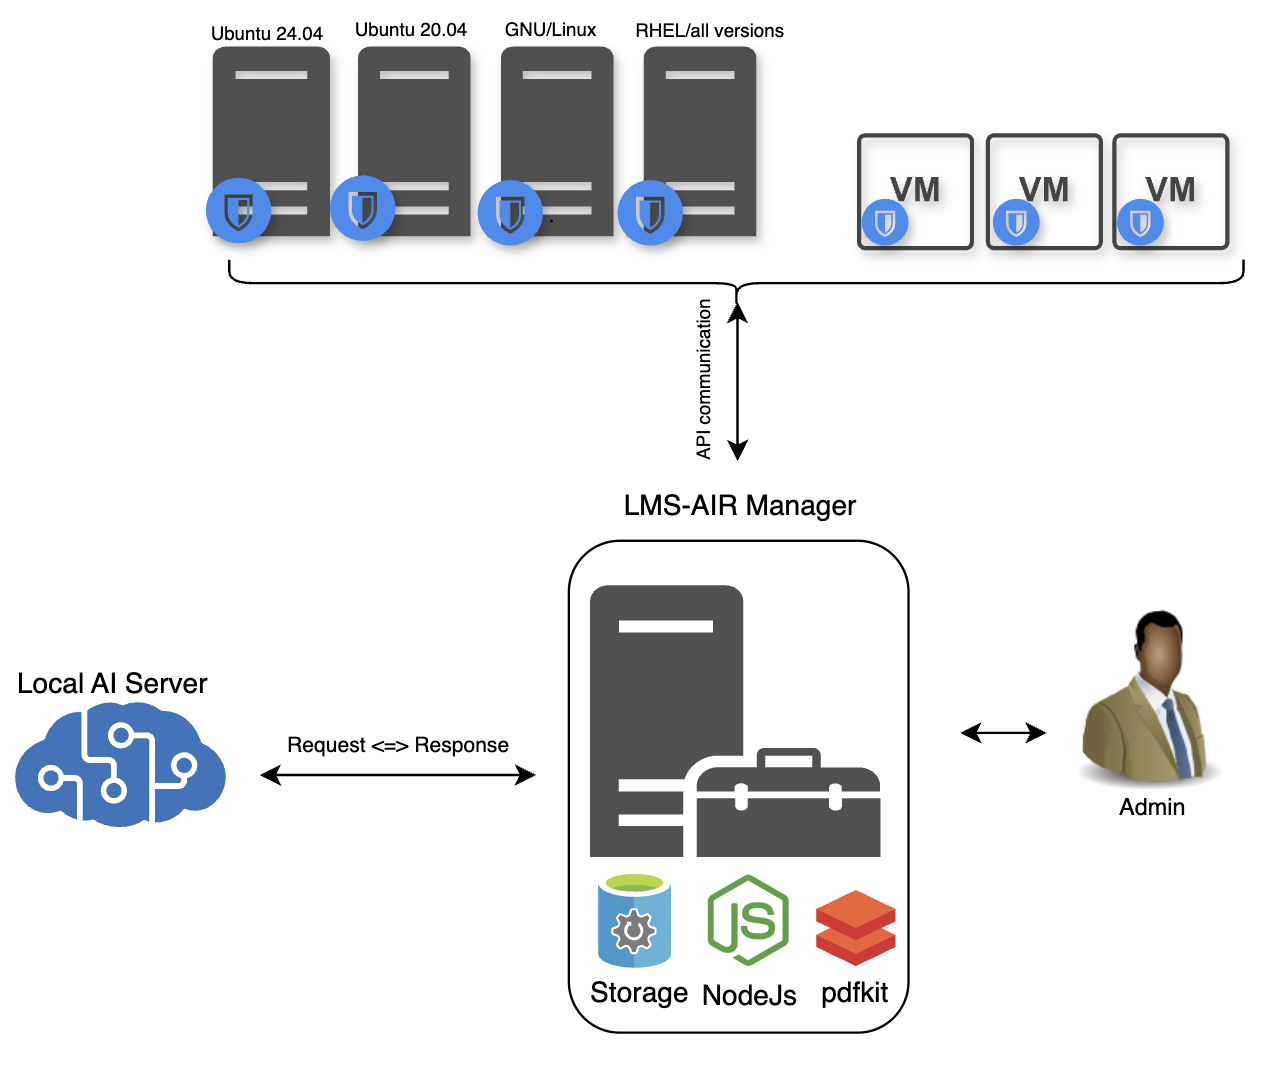
\includegraphics[width=0.6\linewidth]{Screenshot 2025-05-01 at 00.27.18.png}
    \caption{LMS-AIR Architecture}
    \label{fig:enter-label}
\end{figure}


In our implementation, the LMS-AIR Manager runs on an M1 MacBook using Ollama, which supports a variety of AI models (Gemma, Phi4, Mistral, Llama 3.2). After evaluating performance and resource consumption, I selected Mistral and Gemma (Google’s Gemini Local AI) for their optimal balance of dataset richness and speed—Phi4, while comprehensive, proved too resource-intensive for real-time analysis. These models power two key services


\begin{enumerate}
    \item \textbf{Security Reporting:} Automated analysis of log data to generate detailed security reports on demand.
    \item \textbf{AI Technical Support Chat:} Users can upload log files and pose questions directly to the AI, which guides deeper troubleshooting efforts.
\end{enumerate}
To maintain continuous oversight, the Agent and Manager communicate via a heartbeat mechanism: the Agent sends an “online” signal when active and an “offline” signal immediately before shutdown. If connectivity is lost, the Agent caches collected data in temporary memory and automatically forwards it upon reconnection. This ensures no data is lost during network interruptions, preserving consistency and reliability throughout any investigation.


\subsection{Agent} 
The LMS-AIR agent is a critical component and the core of the Log Management System (LMS), serving as the first line of defense for Linux Debian servers. Built in Python, it operates in real-time, leveraging high-speed processing to monitor, analyze, and respond to security events. The agent integrates with rsyslog, which writes system logs to files such as /var/log/auth.log, enabling the agent to process these logs efficiently. It performs multiple tasks concurrently, including log collection, real-time forwarding to a central manager, threat detection using both rule-based and machine learning (ML) methods, and immediate response actions. The agent’s primary focus is on security, particularly in authentication, ensuring rapid detection of brute force attacks and identifying legitimate users. It monitors brute force attempts across three time windows (1, 5, and 10 minutes) to catch both fast and slow attacks, countering attempts by attackers to evade detection through delayed tactics.

The agent maintains a constant connection with the manager to forward parsed log entries and status updates. In the event of a connection loss, it continues to protect the server autonomously by storing all log entries in memory without any limit, ensuring no data is lost. Once connectivity is restored, the agent sends all buffered logs to the manager and clears the memory buffer to optimize resource usage, addressing the consistency requirement for comprehensive log availability. This approach supports deep data analysis by ensuring every log is accessible for investigation.

The agent’s architecture comprises three main components:

\begin{enumerate}
    \item \textbf{Log Management Component}: This component collects logs from rsyslog-generated files, parses them into structured data (e.g., timestamp, source IP), and forwards them to the manager via HTTP POST requests. It uses multithreading to tail multiple log files simultaneously and buffers logs in memory during manager downtime, sending them once reconnected and freeing memory afterward.
    \item \textbf{Threat Detection Component}: Focused on identifying threats, this component analyzes logs using rule-based thresholds (e.g., more than 5 SSH login failures in 1 minute) and a RandomForestClassifier ML model to detect patterns like brute force attacks or port scans. It processes data across multiple time windows to ensure both rapid and prolonged attacks are caught, enhancing security for authentication processes.
    \item \textbf{Response Component}: Upon threat detection, this component blocks malicious IPs using iptables and sends alerts to the manager. It generates threat-specific log entries and status updates, ensuring rapid mitigation and notification. Alerts are buffered during offline periods, maintaining communication integrity.
\end{enumerate}

The agent is fully built with Python and uses port 3000 to forward, communicate with the manager. To solve the inconsistency in case of a manager failing, there is the Global Buffer this help by storing data temporary once the agent is reconnected to the manager logs will be sent to the manager and if something happen that the agent is not able to send the log to the manager, the agent will attempt later to resend once it fully send the agent will free the storage so the manager will have nothing to lose because the data collection is unlimited once everything get back together.  The agent is not just made to monitor the server, but it provides protection as well and defends the server under attack and many different things
\begin{figure}
    \centering
    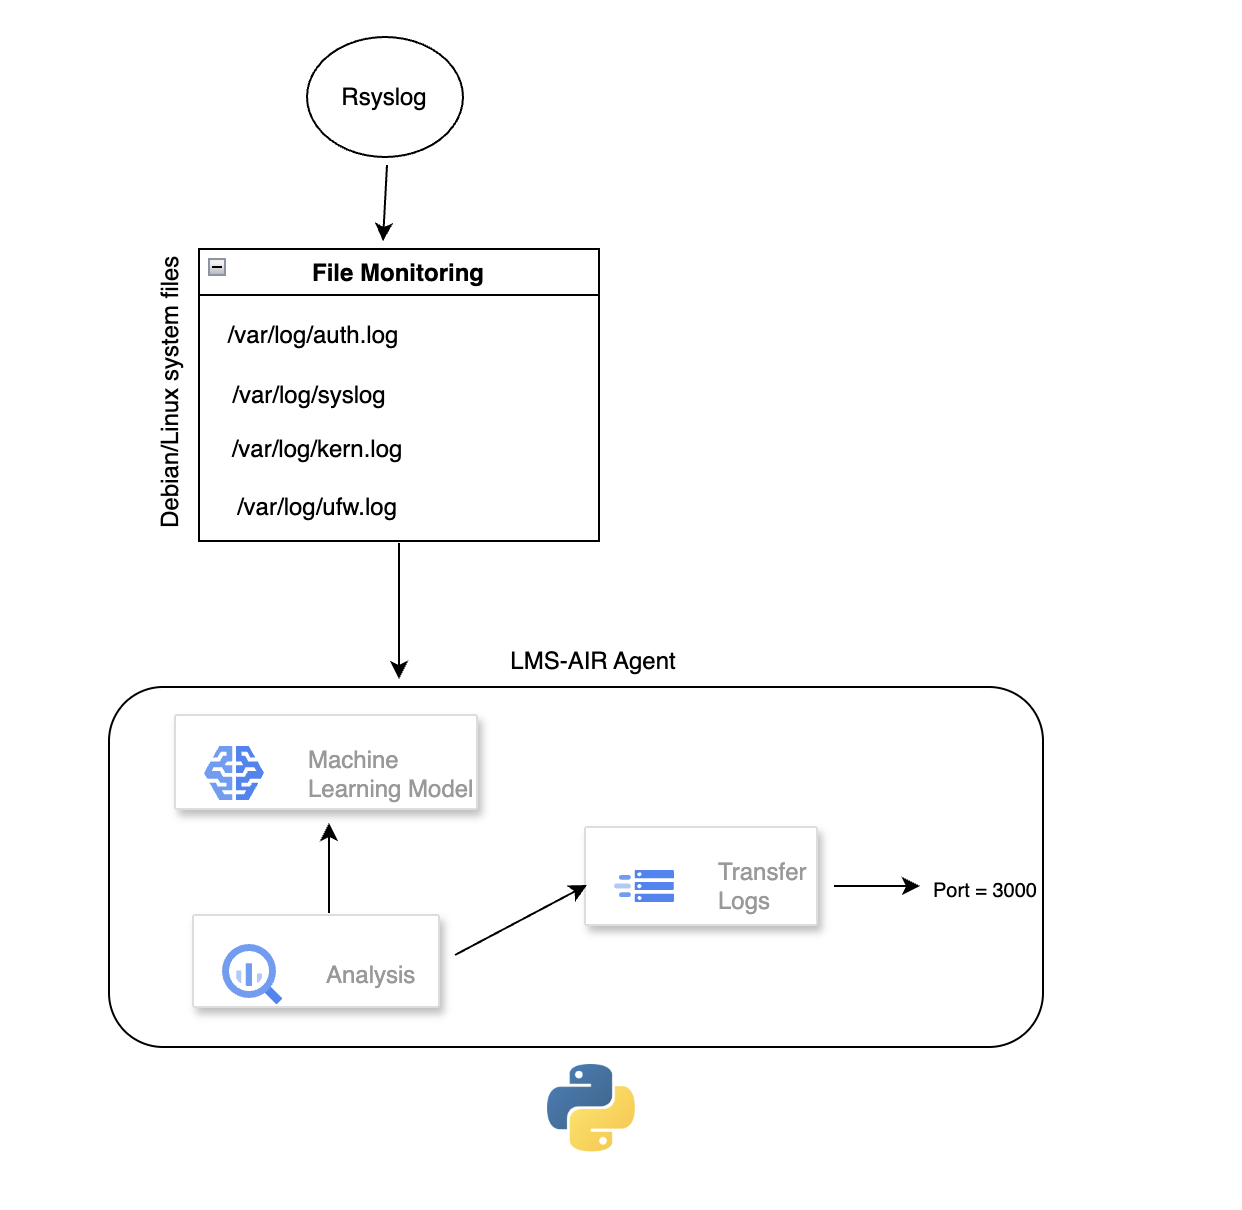
\includegraphics[width=0.5\linewidth]{Screenshot 2025-04-29 at 20.00.14.png}
    \caption{Agent Architecture}
    \label{fig:enter-label}
\end{figure}


\textbf{Agent features}

The LMS-AIR agent extracts a set of features from log data to enable robust threat detection, as defined in the FEATURES constant: ssh\_failed\_1min, ssh\_failed\_5min, ssh\_failed\_10min, sudo\_failed\_1min, sudo\_failed\_5min, sudo\_failed\_10min, root\_logins\_1hr, root\_logins\_24hr, port\_attempts\_1min, port\_attempts\_5min, port\_diversity, and time\_of\_day. These features are computed by the extract\_features function, which processes the threat\_data dictionary tracking events like SSH failures, sudo failures, root logins, and port scans per IP. Each feature plays a specific role in identifying patterns indicative of threats, feeding into both rule-based and machine learning-based detection mechanisms. Below is a detailed explanation of each feature, presented separately.

\textbf{ssh\_failed\_1min}: This feature counts the number of failed SSH login attempts from a specific IP within the last minute. The extract\_features function calculates it by iterating through the ssh\_attempts[1] list in threat\_data, which stores timestamps of SSH failures (triggered by log lines containing "Failed password" or "Invalid user"). Only attempts within the 60-second window from the current time are counted. This feature is critical for detecting rapid brute force attacks, as a high value (e.g., exceeding the THRESHOLD of 5) triggers immediate rule-based alerts and informs the RandomForestClassifier model to predict threats, enabling swift response to aggressive authentication attacks.

\textbf{ssh\_failed\_5min}: This feature measures failed SSH login attempts from an IP over a 5-minute window. Computed similarly to ssh\_failed\_1min, it uses the ssh\_attempts[5] list, counting timestamps within 300 seconds of the current time. By extending the observation period, it captures slightly slower brute force attempts that might evade shorter-term detection. This feature enhances the agent’s ability to identify persistent but less aggressive attacks, contributing to both rule-based checks (e.g., in train\_model for labeling brute force) and ML predictions, ensuring comprehensive coverage of authentication threats.

\textbf{ssh\_failed\_10min}: This feature tracks SSH login failures over a 10-minute window, using the ssh\_attempts[10] list to count attempts within 600 seconds. It targets slow and stealthy brute force attacks, where attackers spread attempts to avoid detection. In train\_model, a high ssh\_failed\_10min value (e.g., > THRESHOLD) labels data as brute force for ML training. Combined with shorter windows, it provides a multi-temporal perspective, allowing the agent to detect varied attack patterns through both rule-based thresholds and ML analysis, bolstering security against prolonged threats.

\textbf{sudo\_failed\_1min}: This feature counts failed sudo authentication attempts within a 1-minute window, derived from the sudo\_attempts[1] list in threat\_data. It processes log lines with "sudo:" and phrases like "incorrect password" or "authentication failure." A high count indicates potential unauthorized privilege escalation attempts. Used in ML model training (e.g., labeling as sudo\_failure if > 3 in 10 minutes), it helps detect anomalies in user behavior, feeding into the RandomForestClassifier to identify threats distinct from SSH-based attacks, enhancing the agent’s focus on authentication security.

\textbf{sudo\_failed\_5min}: This feature tracks sudo authentication failures over a 5-minute window, using the sudo\_attempts[5] list to count attempts within 300 seconds. It complements sudo\_failed\_1min by capturing slightly prolonged attempts to misuse sudo privileges. In extract\_features, it contributes to feature vectors for ML predictions, enabling the model to differentiate between normal user errors and malicious patterns. By monitoring longer-term sudo misuse, it strengthens the agent’s ability to detect persistent privilege escalation attempts, supporting both ML and rule-based detection.

\textbf{sudo\_failed\_10min}: This feature counts sudo failures over a 10-minute window, using sudo\_attempts[10] timestamps within 600 seconds. It targets slow, deliberate attempts to guess sudo credentials, which might indicate an insider threat or compromised account. In train\_model, a threshold (> 3) flags sudo failures for ML labeling. This feature enhances the agent’s sensitivity to extended malicious behavior, feeding into the ML model to predict sudo\_failure threats, ensuring comprehensive monitoring of authentication-related risks.

\textbf{root\_logins\_1hr}: This feature counts successful root login sessions within the last hour, derived from root\_logins in threat\_data, which records timestamps of "session opened for user root" events. Calculated by checking entries within 3600 seconds, it helps detect unusual root activity, especially when combined with time\_of\_day (e.g., root logins at odd hours). In train\_model, > 2 logins in 1 hour during early morning hours flags a root\_anomaly. The ML model uses this to identify potential privilege misuse, enhancing security for critical accounts.

\textbf{root\_logins\_24hr}: This feature tracks root logins over a 24-hour period, counting root\_logins entries within 86400 seconds. It provides a broader context for root activity, identifying patterns of excessive access that might indicate compromised credentials. Used in extract\_features for ML feature vectors, it helps the RandomForestClassifier distinguish normal administrative behavior from anomalies. By monitoring long-term root access, it supports the agent’s focus on securing high-privilege accounts, complementing shorter-term detection.

\textbf{port\_attempts\_1min}: This feature counts port scan attempts from an IP within a 1-minute window, using port\_attempts[1] from UFW logs (e.g., lines with source IPs and ports). It captures rapid probing of network services, a common reconnaissance tactic. Calculated in extract\_features, a high count (> 10 in 5 minutes in train\_model) flags port scans. This feature informs ML predictions and rule-based checks, enabling the agent to detect network-based threats early, protecting the server from potential exploitation.

\textbf{port\_attempts\_5min}: This feature tracks port scan attempts over a 5-minute window, using port\_attempts[5] to count entries within 300 seconds. It identifies sustained scanning efforts that might be less intense but still malicious. In train\_model, combined with port\_diversity, it labels data as port\_scan if both are high. The ML model uses this to detect prolonged reconnaissance, enhancing the agent’s ability to counter network threats that evolve over time, ensuring robust perimeter security.

\textbf{port\_diversity}: This feature measures the number of unique ports targeted by an IP, derived from the ports set in threat\_data, populated by parsing UFW log lines (e.g., with "DPT=80"). A high value indicates broad scanning across services, a hallmark of reconnaissance. In train\_model, port\_diversity > 5 with high port\_attempts\_5min flags port scans. The ML model leverages this to identify sophisticated attacks, complementing port attempt counts to distinguish malicious scanning from legitimate traffic, strengthening network threat detection.

\textbf{time\_of\_day}: This feature represents the time of an event in minutes past midnight, calculated in extract\_features using the current time’s hour and minute (tm\_hour * 60 + tm\_min). It contextualizes events, as certain activities (e.g., root logins at 2 AM) are more suspicious. In train\_model, it flags root\_anomaly if root\_logins\_1hr > 2 and time\_of\_day < 360 (6 AM). The ML model uses this temporal context to enhance anomaly detection, improving the agent’s ability to identify unusual behavior across all threat types.




%     \centering
%     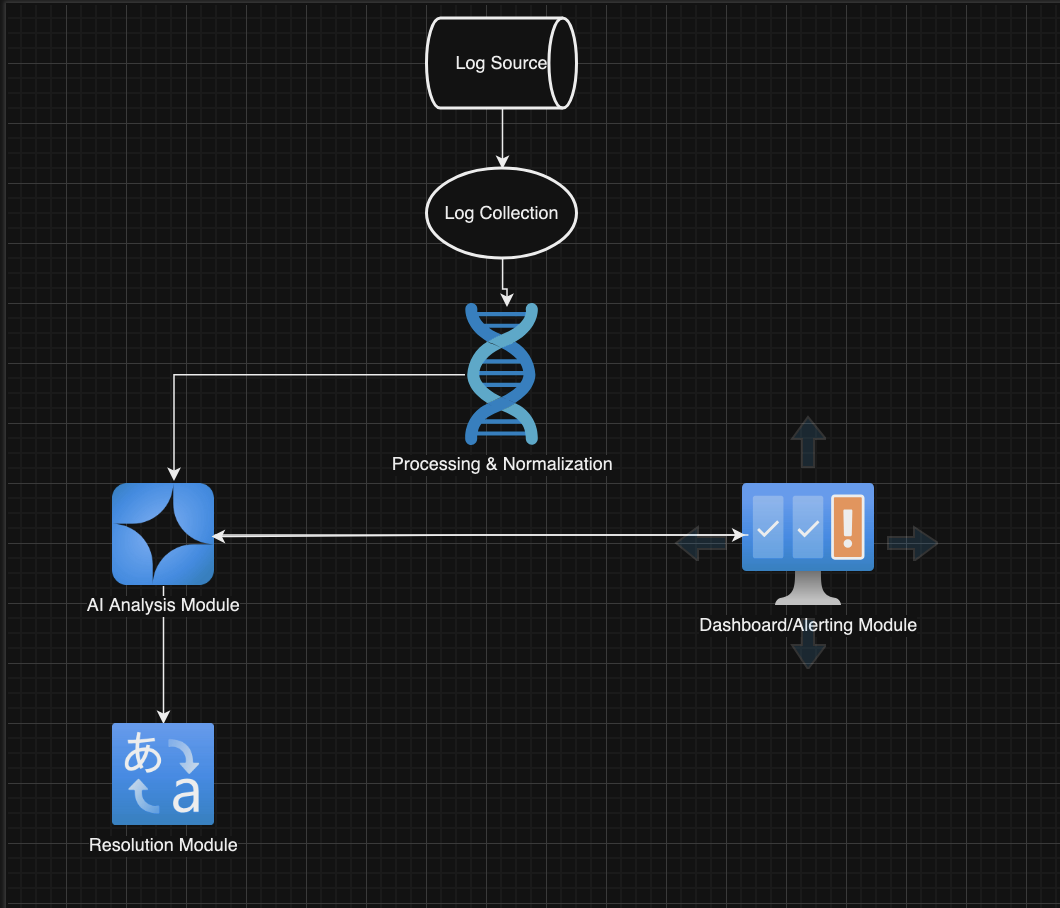
\includegraphics[width=0.75\linewidth]{Screenshot 2024-11-26 at 19.12.15.png}
%     \caption{Enter Caption}
%     \label{fig:enter-label}
% \end{figure}





% Describe the architecture of the solution that you have in mind, including:
% \begin{itemize}
%     \item Technologies involved (e.g., frameworks, programming language). 
%     \item The hardware needed to develop the project (and to support at deployment stage)
% \end{itemize}

% For the project to be completed I'll have to use a my personal PC running with 3 Virtual Machines, The 3 VMs will send their logs to the host server, that is where I'll be running the application. 




\subsection{Manager}

\textbf{Initialization \& Directory Setup}

On startup, the manager ensures the file system is ready to receive and organize data. It creates three primary directories—machine_logs/ for raw log entries from agents, threats_detected/ to isolate only those entries flagged as threats, and reports/ for storing generated PDF security analyses. It also loads (or initializes) a machines.json file, which acts as a lightweight registry tracking each machine’s hostname, IP address, last‐seen timestamp, and online/offline status.

\textbf{Core Middleware \& Utilities}

The Express application layer is configured with essential middleware: CORS to permit cross‐origin requests, Morgan for HTTP request logging, body parsers for JSON and URL‐encoded payloads, Multer for handling file uploads, and CookieParser. Static assets are served from the public/ folder, and EJS is set as the templating engine for server‐rendered views. A simple logging middleware stamps every incoming request with a timestamp, method, and URL to the console.

\textbf{Machine Status Tracking}

Agents report their health and status via POST /api/status. When a new machine registers, its metadata (hostname, IP, status) is written to machines.json. Subsequent heartbeats update the last_seen timestamp and may include an alert field—if present, that alert is appended to the machine’s log file. Separately, a background timer runs every minute to detect machines that have been silent for more than 15 minutes, automatically marking them offline and writing an “offline due to inactivity” entry into their log.

\textbf{Log Ingestion \& Storage}

Raw log events arrive at POST /api/logs in JSON format. The manager updates the reporting machine’s last_seen timestamp and appends each entry either to machine_logs/<machine_id>.log (for routine entries) or to threats_detected/threat_machine_<machine_id>.log (for entries where log_type === "threat_detected"). This file-based approach gives a persistent, per‐machine history of both benign and potentially malicious activity.


\textbf{Threat Retrieval}

To review only the flagged incidents, clients can call GET /api/threats/:machine_id. The manager reads and parses the corresponding threat log file and returns an array of JSON entries. If no threat log exists or is empty, it responds with a friendly “no threat logs found” message, ensuring the UI or API consumer can handle both cases gracefully.
DeepSearch Analysis \& PDF Reporting

For in-depth, AI-driven security audits, GET /api/deepsearch/:machine_id loads up to the most recent 500 (It can go higher then this is just because my own computer won't support that much pressure )log lines for a machine, wraps them in a system/user prompt, and sends that to an Ollama-powered LLM (e.g. mistral:latest). The text report returned is streamed into a PDF via pdfkit—complete with header, generation timestamp, and the body of the analysis—and saved under reports/. The endpoint returns both the raw text report and URLs for inline viewing or direct download of the PDF.

\textbf{Ad-Hoc Chat Endpoint}

The POST /chat route supports interactive, on-demand log analysis. It accepts either a multipart upload (logFile) or a JSON array of chat messages. A fixed “system” prompt identifying the service as the LMS-AIR agent is prepended, and the combined message set is forwarded to Ollama. Responses can be streamed via Server-Sent Events or returned as a single JSON payload, enabling flexible integration in UIs or scripts.
% UI Routes

A simple dashboard is exposed via GET /Mevents?machine_id=…, rendering an EJS template that displays machine metadata (status, hostname) alongside its parsed logs. If the machine is offline, the page notes that but still shows historical entries. Static files, including client-side scripts and styles, live under public/, and generated PDFs can be viewed inline (/reports/view/:filename) or downloaded (/reports/download/:filename), supporting both ad-hoc and scheduled reporting workflows.




























% Provide a high level view of the system you have in mind, including any package of classes, what is it responsible for and what other packages it communicates to. Provide a high level view of the database (or structure) needed to support the project, including what each table/document is responsible for and the hierarchy among them. You need to be as specific here as you can, why? Because this will aid you in identifying parts of the project you are vague on, this may be fine for some components but cause problems in term 2 for others. If you have hardware element in your project this is also where you provide a high level view of how these elements integrate into the project. So for a project that is cyber-physical you will have both a hardware and software architectural diagram. N.B. This is NOT a full system design but a high level overview of what you can credibly develop. This architecture should be informed by prototyping activity. 

% Some of the implementation focused projects may describe how do you envision tackling the functional requirements of your project via a set of use-cases. DFDs are also helpful here to understand elements of your project that may cause problems. You should describe the role of the different parts of the architecture of the solution, and the interaction among them.

\section{Risk Assessment}
% Identify any potential risk precluding you from successfully complete your project. This section is really important and often neglected by students resulting in fatal risks occurring in some projects. Make sure to give this section the time it requires. Classify the risk according to their importance, possibility of arising and enumerate the decisions you can make to anticipate them or mitigate them (in case they finally arise). Table \ref{tab:ProjRisks} may help with this classification. This section should include your mitigation approach for any critical risks.

    \textbf{1. Inconstant Timestamp}


One of the problems can happen is the timestamp, For example 2 different servers sending logs with 2 different timestamps that can damage the accuracy of the log monitoring and can lead to a false positive. timestamps can break correlating rules, causing the manager to miss critical patterns. if logs are delayed due to a network issue that can make it difficult to reconstruct events accurately.


To solve this issue running Network Time Protocols will be the solution by synchronising all data timestamps so their clock will be reliable, I will configure an NTP server in all of the clients using a standard timezone logs to avoid timezone-related discrepancies 


\textbf{2. Failure of the Manager}



The agent install on the server will keep monitoring logs as normal and will keep every thing in the global buffer to be resend later once the manager is back and this will keep the system to be monitoring if the connection between the manager and agent is not working an alert will be send to the client  via email to alert the administrator about the incident so it can be fix as soon as possible.



\textbf{3. Operating Systems Deployment}


The operating system is something important for this project to work just for clarification this project is mostly focused on Unix/Linux operating systems, the device I have and that I'll build the software  Linux but the issue will be to transfer logs via networks is a bit complex but it's doable.


\textbf{4. Miss-configuration  of the system}


A misconfiguration of a system can cause damage and inconsistency on data processing, devices must match the requirements for better performance. a KB will be on the manager side to show how the installation process will be to help the user to deploy the system safely and avoid all types of problem may occur in the process 


\textbf{5. Failure of the agent/ Agent offline}


In case of agent failure, the log will not be received, leading to inconsistent or log collections. There is a mechanism that will be set to the manager by telling if the agent is offline and the user will be notify that the agent is offline that can help the administrator to detect the problem and get things back on track


\begin{table}[h]
\centering
\scriptsize
\caption{Initial risk matrix}
\begin{tabular}{|p{2cm}|p{2cm}|p{2cm}| p{2cm} |p{2cm}| p{2cm}|}
\hline \bf Frequency/ Consequence & \bf 1-Rare & \bf 2-Remote & \bf 3-Occasional & \bf 4-Probable & \bf 5-Frequent\\ [10pt]

\hline \bf 4-Fatal & \cellcolor{yellow!50} & \cellcolor{red!50} Miss-configuration  of the system & \cellcolor{red!50} & \cellcolor{red!50} &\cellcolor{red!50} \\ [10pt]

\hline \bf 3-Critical &\cellcolor{green!50} Failure of the Manager & \cellcolor{yellow!50} Inconstant Timestamp & \cellcolor{yellow!50}  & \cellcolor{red!50} &\cellcolor{red!50} \\ [10pt]

\hline \bf 2-Major & \cellcolor{green!50} & \cellcolor{green!50} & \cellcolor{yellow!50} &\cellcolor{yellow!50} Failure of the agent/ Agent offline &\cellcolor{red!50} \\ [10pt]

\hline \bf 1-Minor & \cellcolor{green!50} & \cellcolor{green!50} & \cellcolor{green!50}  Operating Systems Deployment &\cellcolor{yellow!50} &\cellcolor{yellow!50} \\ [10pt]
\hline
\end{tabular} \\
\label{tab:ProjRisks}
\end{table}







\section{Methodology}
% Describe your personal approach on how to tackle the different parts of this project, including:


% \begin{itemize}
%     \item How to tackle the needed research to fulfill the background chapter. 
%     \item How to set up your Computer Science skills to the project needs (e.g., describe your plan to learn any new technology involved on the project that you are not familiar with). 

The whole project is a mixed up of different field in computer sciences here we can find Cybersecurity, IT Management, AI/Machine learning all combine to build a light weight application that can solve monitoring problems. the research really opened up my eyes in different areas of computer sciences to find good or bad form monitoring systems.  

\textbf{1. Research}

The plan is to keep learning more as the project AI/Machine learning is involved those areas are new to me so it a big boost to learn more and go deeper into my search. My focus will be more on research papers and through the internet about some specific subject that can benefit the project also there are some tutorial on YouTube that will be a big help to develop new skills, keep researching into existing log monitoring systems understand their limitations, and identifying areas where AI can provide significant improvement as the research will involve studying the best practices in Cybersecurity and AI-driven solutions for security threat detection. Specifically, I will explore how AI techniques like anomaly detection, pattern recognition, and natural language processing can be applied to log data to detect potential security incidents.

\textbf{2. Skill Development}


Since AI and Machine Learning are new areas for me, I will dedicate a significant portion of my time to learning the fundamental concepts of these technlogies. This will involve taking online course in YouTube, studying some case studies related to AI in cybersecurity. I will focuss on understanding commonly used in security spplications, such as supervised learning, unsupervised learning, and reinforcement learning, to apply them to log data for intelligent decision-making 


\textbf{3. Log Data Analysis}

I will analyse various types of log data to identify patterns and anomalies that indicate potential security threats. This will involve prepocessing the logs to clean and format the data, followed by exploring different AI models to clasify and predict security issues based on historical log data.


\textbf{4. System Development}


The next step will involve implementing the AI-driven log monitoring system. I will integrate machine learning algirithms with the log data to build a model that can automatically detect suspecious behaviour, unauthorized access, or other security risks. This system will use the learning pattern from the logs to generate real-time aleart and recommend automated responses to the user.


\textbf{5. Testing and Evaluation}

Once the system is developed, I will test using real or simulated log data to evaluate its effectiveness in detecting security threats. I will assess the system's performance based on key metrics such as accuracy, precision, recall, and response time. Based on the results, I will interactively improve the AI models and the overall system design to optimize security performance.


%     \item What core project managing approach will you follow (e.g., Waterfall, Scrum, etc).
% \end{itemize}

\section{Implementation Plan Schedule}
Come up with a schedule for the remaining time (including second semester), so as to describe how do you envision to achieve the implementation of your project by the end of semester 2. This plan SHOULD be ambitious but MUST be realistic and SHOULD be informed by early prototyping and MUST be discussed with your term 1 supervisor.

\textbf{Phase 1 Infranstructure set up}

The Infranstructure is something I have to take in consideration as I was able to Install and run ELK on my machine, it was working fine until I endup with resources issue the machine I used is a Core i5 8GB this is unable to run ELK and 2 virtual machine running at the same time the machine was frozen, this phase can take me one week to arranged everything as If I use macbook for the project I will need to find a workaourd way to transfer logs from Virtual Machines to the Mac this, a windows is not an option for what I have not a single programme will run well.


\textbf{Phase 2 Model Development \& Trainning 1 to week 3 }

During this phase, I will focus on developing the machine learning models required for log anomaly detection, classification, and root cause analysis. I will need to train these models using historical log data, ensuring that the models are capable of identifying patterns and anomalies effectively. I will implement both supervised and unsupervised learning techniques depending on the availability of labeled data. The models will be tested to evaluate their accuracy and performance, and I will refine them by fine-tuning parameters and adjusting features. I will also need to handle the challenges of log data variability, ensuring that the model can handle different formats, and optimize the performance of the model for real-time processing. Once the models are ready, I will validate them against test datasets and establish performance metrics to gauge their effectiveness.


\textbf{Phase 3 Model Development \& Training 3 to week  6}

In this phase, I will integrate the trained AI models into the log monitoring system. I will ensure that the models can analyze logs in real-time and accurately detect anomalies or issues. I will need to implement an automated resolution mechanism based on the detected anomalies, which might include actions such as service restarts, alert generation, or corrective tasks. Additionally, I will need to set up the system for root cause analysis by correlating logs from different sources and generating insights. Testing will be a crucial part of this phase, as I will need to verify that the system performs as expected in real-world conditions. I will conduct end-to-end tests to evaluate the speed, accuracy, and reliability of the entire system, ensuring that both the AI models and the automated actions function properly in various scenarios.

\textbf{Phase 4 Testing 6 to week 7}
This phase will be focus on testing I'll spend a whole week testing the system to try to find what I need to fix and rule I would need in the future to make the project successfully. the test will involve some attack to Virtual Machine and see how the system will react checking all alerts and what needed for the project to reach the goal.

\textbf{Phase 5 Deployment \& Rollout 7 to week  9}

During this phase, I will deploy the AI-driven log monitoring system in a staging environment to simulate real-world log data and assess its performance. I will need to perform stress tests to ensure the system can handle high volumes of log data without compromising on performance. Once the staging tests are successful, I will roll out the system to the production environment. This will involve migrating the configuration, models, and tools from the test environment to production while ensuring that the system remains secure, scalable, and reliable. I will also need to set up a monitoring dashboard to visualize logs, anomalies, and system health. The dashboard will allow system administrators to interact with the data and monitor the resolution processes. The final deployment will ensure that the system is ready for continuous operation.


\textbf{Phase 6 Post-Deployment Monitoring}


Once the system is deployed and running in production, I will continuously monitor its performance and effectiveness. I will need to track the accuracy of the AI models, the system’s ability to detect and resolve issues, and any new challenges or areas for improvement. Post-deployment, I will gather feedback from users and stakeholders to refine the models and optimize the system. If the volume of logs increases or new sources are added, I will need to scale the infrastructure to accommodate this growth while maintaining performance. Additionally, I will regularly update the AI models with new log data to improve their accuracy and adapt to changing patterns. This ongoing optimization process will ensure that the system remains effective, responsive, and reliable over time.

 \section{Evaluation}
% Come up with an evaluation plan that allows you to measure how much have you actually achieved the goals of your project. This again is a section that is often neglected where students loose marks. How do you plan to measure the output of your project? A binary it works/does not work is insufficient. You need to be able to quantify the success against both the functional requirements and the initial idea. These are not the same as you may meet all function requirements outlined but not solve the overall problem because you have failed to revisit these and update them with new information which you learn as you are developing the project.
To effectively evaluate the success of the AI-driven log monitoring system and determine how much the project has achieved its goals, Here a comprehensive evaluation plan to implemented. This plan will measure success based on both functional requirements and the initial goals outlined in the project proposal, to ensuring that the system addresses the core problem while meeting technical specifications. The evaluation will include both quantitative and qualitative assessments, providing a clear picture of the system’s effectiveness and areas for improvement. This will go beyond a simple "works or doesn’t work" approach, and will offer insights into the system's actual performance and value.




\subsection{Functional Requirements Evaluation}

The functional requirements describe the technical capabilities that the system must fulfill, and evaluating how well these are achieved will be crucial for determining the success of the project. This evaluation will assess each core function, ensuring that the system performs as expected in real-world environments.

\textbf{1. Log Collection and Integration}


In the first step, I will assess whether the system can collect logs from multiple sources, such as servers, applications, and databases. This includes checking the integration of log collection rsyslog with existing systems. The key metrics for evaluating success in this area include the log collection rate, which measures how quickly and in what volume logs are collected, and log integrity, which examines whether logs are transferred accurately without data loss or corruption. The integration success rate will also be important, tracking the percentage of sources successfully integrated into the system. These metrics will be tested using automated simulations that mimic the real-world environment, followed by manual checks to ensure data integrity.



\textbf{2. Log Parsing and Structuring}


The system must correctly parse and structure raw log data into usable formats for analysis. In this phase, I will evaluate the parsing accuracy, which measures how well the system transforms raw log data into a structured format such as JSON or key-value pairs. Additionally, the data loss percentage will be tracked to identify any logs that fail to parse correctly due to formatting issues. This evaluation will be conducted by comparing the parsed logs against manually verified data samples.

\textbf{3. AI Model Accuracy and Performance}


A central aspect of the project is the development and deployment of AI models capable of detecting anomalies, classifying logs, and performing root cause analysis. To measure the success of this function, I will focus on anomaly detection accuracy using precision, recall, and F1-score metrics. Additionally, the false positive rate will be important to evaluate how often normal logs are mistakenly flagged as anomalies. Classification accuracy will assess the system's ability to categorize logs into predefined categories (e.g., error, warning, info). Lastly, root cause analysis accuracy will measure how well the system identifies the source of the issue from correlated logs. These metrics will be determined using confusion matrices and cross-validation on labeled datasets, with real-world testing ensuring that the system can effectively analyze live log data.



\textbf{4. Automated Resolution and Actions}


The system’s ability to automatically resolve or respond to detected anomalies will be evaluated by assessing the action success rate, which measures how often the system’s automated responses (e.g., restarting services, sending alerts) are successful in mitigating issues. The resolution time will track how quickly the system resolves issues after detecting them, while action appropriateness will ensure that the responses are suitable for the detected problems. These metrics will be evaluated by logging all actions taken by the system during controlled test scenarios and comparing them to the expected results.



\subsection{Addressing the Initial Project Goals}

The initial goal is to improve operational efficiency by automating log monitoring and issue resolution, as well as to speed up detection and resolution processes. These goals will be evaluated through both quantitative and qualitative means.

\textbf{1. Operational Efficiency Improvement}


To evaluate operational efficiency, I will track the reduction in manual intervention and effort required for log analysis and issue resolution. Specifically, I will measure the manual intervention reduction, comparing the number of hours spent on log monitoring and troubleshooting before and after the system’s implementation. Additionally, I will assess the system downtime reduction, measuring how much the automated system reduces the time spent resolving issues that could have been detected earlier. These metrics will be gathered by comparing historical incident records with the post-implementation period, offering a clear picture of operational improvements.



\textbf{2. Detection and Resolution Speed}


The speed at which the system detects issues and resolves them will be a key metric for evaluating the effectiveness of the system. I will measure the detection time, which records the time between an issue occurring and its detection by the system, and resolution time, which tracks the time between detection and issue resolution. By comparing these metrics to industry standards or baseline data from the pre-implementation period, I will evaluate whether the AI-driven system delivers faster detection and resolution than manual processes. Controlled tests will be used to simulate various issues and measure the response times.

\textbf{3. Scalability and Performance Under Load}


Scalability is essential for ensuring that the system can handle increasing volumes of log data over time. In this phase, I will conduct stress testing and load testing to measure how well the system handles increasing data volumes without degradation in performance. Metrics such as throughput, which measures the number of logs the system can process per minute or hour, and system latency, which tracks the time taken to process logs, will help assess the system’s scalability. Additionally, system load handling will test the system’s ability to maintain performance under heavy log traffic or complex log data scenarios. These tests will simulate different operational loads and monitor system performance to ensure it scales effectively.

\textbf{4. Adaptability to Changing Patterns and New Log Sources}


As logs and log sources evolve over time, it is essential that the AI models remain effective. I will measure model adaptation rate, which tracks how quickly the system adjusts to new log formats or sources, and accuracy after adaptation, which evaluates how well the models continue to perform after being adapted to handle new data. This will be measured by introducing new types of log sources or anomaly patterns and assessing the system’s ability to detect and resolve issues associated with these changes.


\textbf{5. Continuous Improvement}


Once the system is deployed, continuous monitoring to ensure ongoing improvements. I will track continuous model improvement by periodically updating the AI models with new log data to ensure they remain accurate and effective in detecting anomalies. This ongoing process will be essential for optimizing the system and ensuring that it adapts to any new challenges that arise over time.
















\section{Prototype}
% Although you do not have a fully functional project yet, you should show wireframes, snapshots or representation on how do you envision your project to look once the implementation phase has been completed. The nature of this section will vary significantly from project to project and can include anything from code snippets to snapshots of service deployments. Any prototyping you have done during the term should be summarized here that has not been captured in earlier sections. For example if you are planning to host your project using AWS in an EC2 instance you should have at least created a "hello world" setup to determine the basics, this probably should have been discussed in section \ref{sec:Arch}.

As you can see on the on this prototype the first host register is Victorious-Latitude-5410 that the second image show logs being monitoring in real-time. at the moment no rules as been each server will have like a profile as the first screenshot show the host name and some main details.

The second screenshots is about got details of each server has you can see some log messages timestamps as I said in the beginning if you click over a line of log you will get more details how the logs is pulled up. 

The last Screenshots is the 2 Virtual Machine I install and there are 2 type of Linux distributor one is Ubuntu Server and the other one is Mint those 2 machine I will use to for the systems.



\begin{figure}
    \centering
    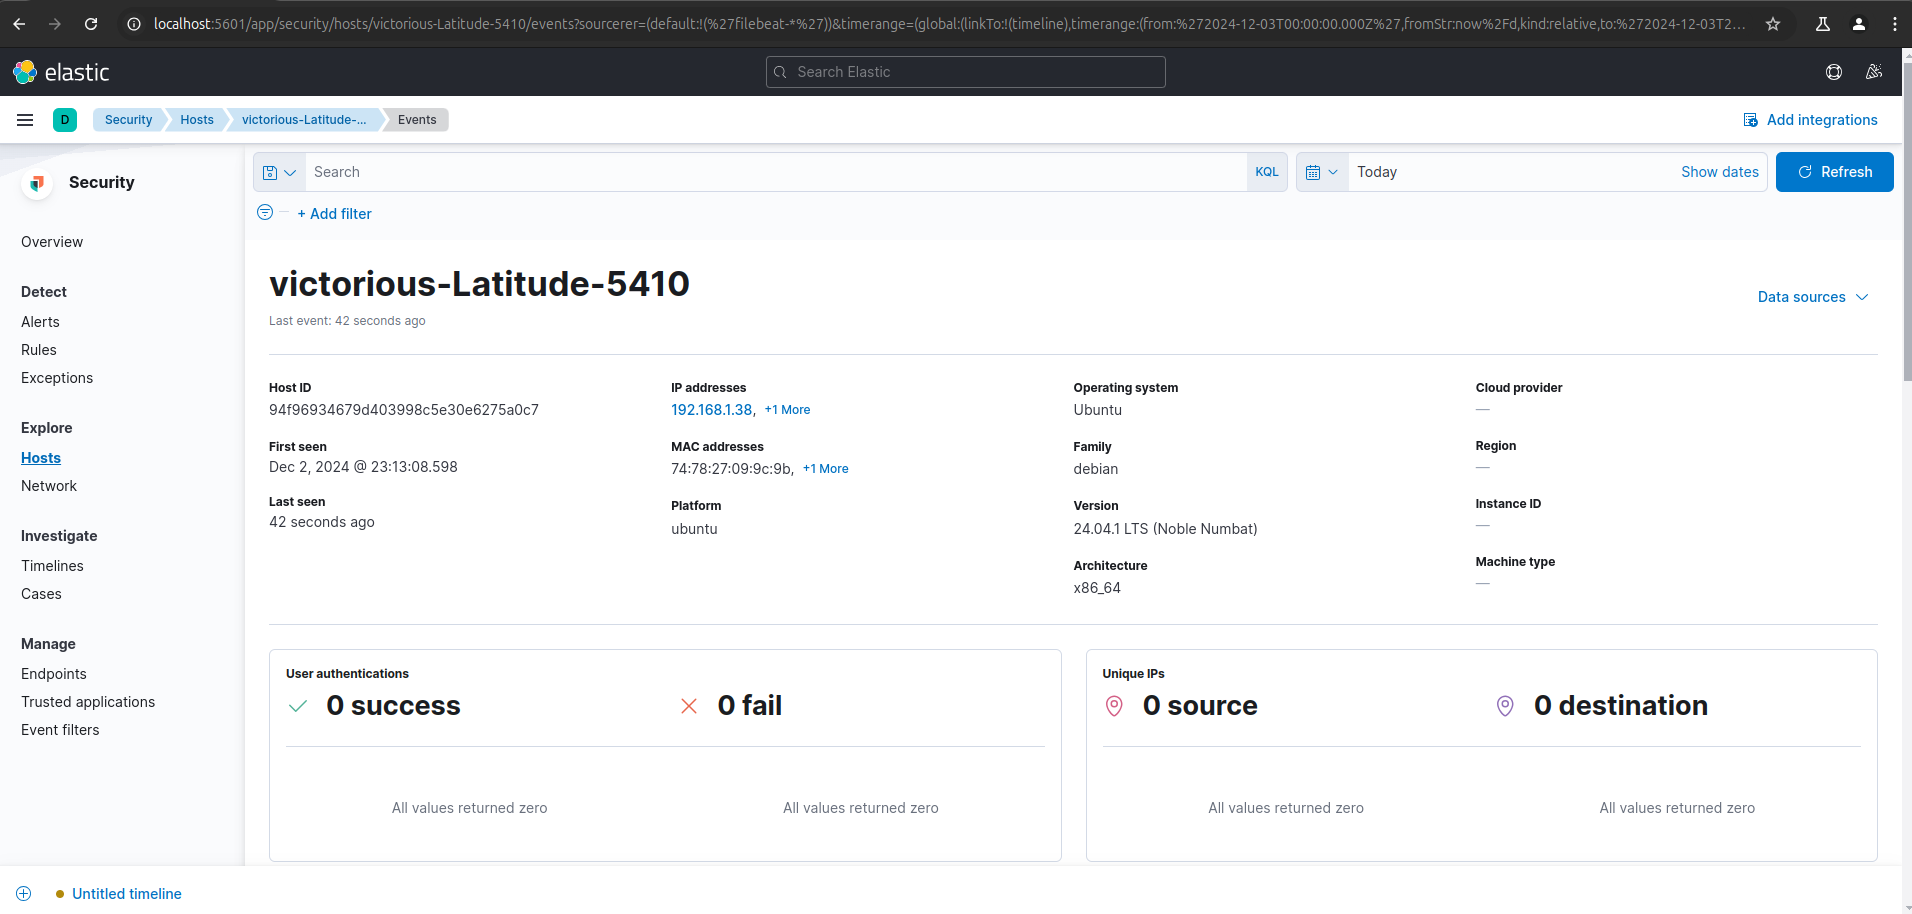
\includegraphics[width=1\linewidth]{Screenshot from 2024-12-03 17-26-16.png}
    \caption{Elastic}
    \label{fig:enter-label}
\end{figure}


\begin{figure}
    \centering
    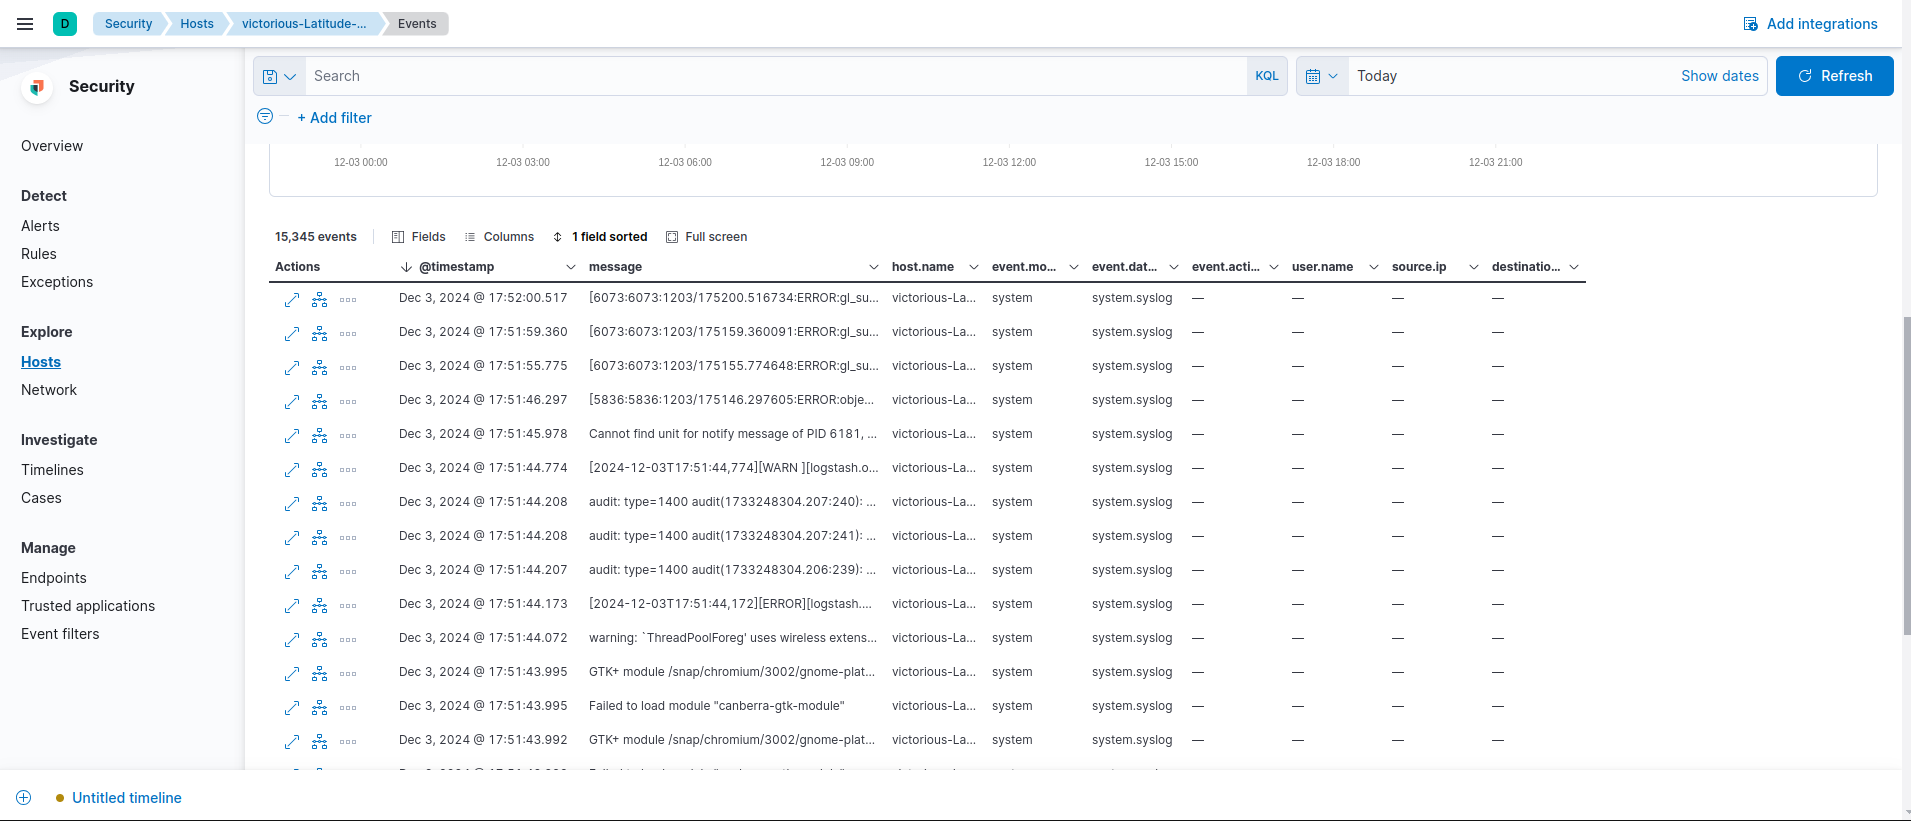
\includegraphics[width=1\linewidth]{image.png}
    \caption{Real-Time Log monitoring}
    \label{fig:enter-label}
\end{figure}

\begin{figure}
    \centering
    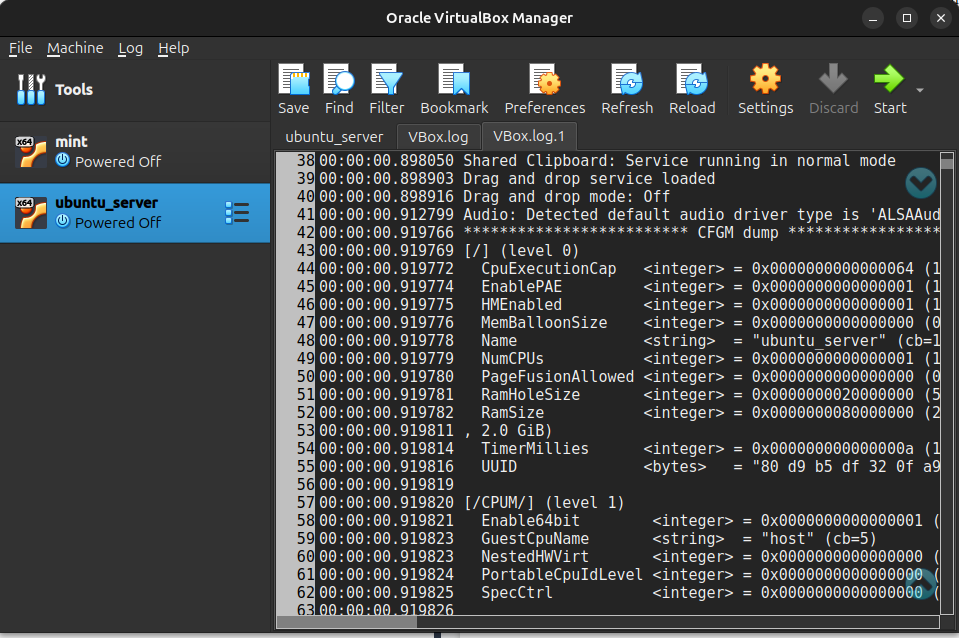
\includegraphics[width=1\linewidth]{Screenshot from 2024-12-03 20-32-39.png}
    \caption{Virtual Machine install}
    \label{fig:enter-label}
\end{figure}
